%%%%%%%%%%%%%%%%%%%%%%%%%%%%%%%%%%%%%%%%%
% Introduction
%
% $Date$
% $Revision$
% $Author$


\chapter{Introduction}\label{chap:introduction}

Modern software applications are often complex and have to fulfill a large set of functional and non-functional requirements. The internal behavior of such large systems cannot easily be determined on the basis of the source code. Furthermore, existing applications often lack sufficient documentation which makes it cumbersome to extend and change them for future needs. A solution to these problems can be dynamic analysis based on application-level monitoring, which allows to log the behavior of the application and to discover, for example, application-internal control flows, calling dependencies, and method response times.

Dynamic analysis can help in detecting performance problems and faulty behavior, capacity planning, and many other areas. The \Kieker{} framework provides the necessary monitoring capabilities and comes with tools and libraries for the analysis of monitored data. \Kieker{} has been designed for %
continuous monitoring in production systems inducing only a very low overhead. Further information on the overhead caused by \Kieker{} is provided at \url{http://kieker-monitoring.net/overhead-evaluation/}.
%, and offline evaluation of monitored data for a deeper inspection of the application's behavior and runtime architecture.

%%
\section{What is \Kieker?}\label{sec:kieker}

\enlargethispage{1cm}

\Kieker{} is a Java-based application performance monitoring and dynamic software analysis framework~\cite{KiekerICPE2012}. %
Monitoring adapters for other platforms, such as Visual Basic~6~(VB6), .NET, and COBOL, exist as well.%
\footnote{\href{http://kieker-monitoring.net/support/}{Contact us} directly if you are interested in \Kieker{} support for other platforms} %
Figure \ref{fig:KiekerComponentDiagram} shows the framework's composition based %
on the two main components \KiekerMonitoringPart{} and \KiekerAnalysisPart{}. %

% This is the component diagram of Kieker (the satellite).
\begin{figure}[H]\centering
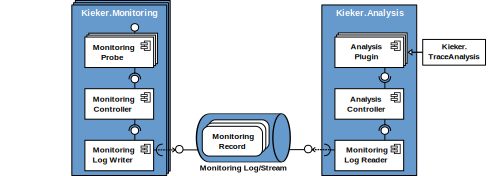
\includegraphics[width=0.96\textwidth]{images/kiekerComponentDiagram-woCloud-bw-w-record-newNames-withTraceAnalysis-colors}
\caption{Overview of the framework components}
\label{fig:KiekerComponentDiagram}
\end{figure}

\noindent The \KiekerMonitoringPart{} component is responsible for program instrumentation, data collection, and logging. Its core is the \class{MonitoringController}. %  which %
%receives the monitoring data in so-called monitoring records from monitoring probes, and writes these %
% receives the monitoring data and passes it to the configured monitoring log writer. %
%
The component \KiekerAnalysisPart{} is responsible for reading, analyzing, and visualizing the monitoring data. Its core is the \class{AnalysisController} which manages the life-cycle of the pipe-and-filter architecture of analysis plugins, including monitoring readers and  analysis filters.

The monitoring and analysis parts of the \Kieker{} framework are composed of subcomponents which represent the different functionalities of the monitoring and analysis tasks. The important interaction pattern among the components is illustrated in Figure~\ref{fig:KiekerCommunicationDiagram} but will be explained furthermore throughout the course of this user guide.

\vspace{1cm}

% This image shows the communication diagram of the different components.
\begin{figure}[H]\centering
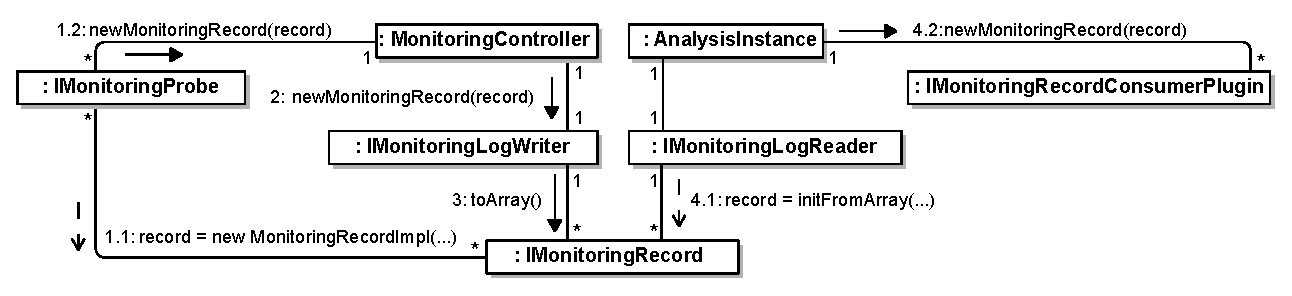
\includegraphics[width=1\textwidth]{images/kiekerCommunications-revisedReArranged-woMonitoringLog-bw-newNames}
\caption{Communication among \Kieker{} framework components}
\label{fig:KiekerCommunicationDiagram}
\end{figure}

% \vspace{1cm}

% Notify-tag because it is explained how Kieker works.
% avh: removed
\noindent The monitoring probes create the monitoring records containing the %
monitoring data and deliver them to the monitoring controller. %
The monitoring controller employs the monitoring writers to write these %
monitoring records to a monitoring log or stream. %
For analyzing purposes, monitoring reader plugins read the records from the %
monitoring log/stream. These records can then be further processed by a %
configuration of additional filter and repository plugins, inter-connected via input and output ports. %

\section{Framework Components and Extension Points}

\begin{figure}\centering
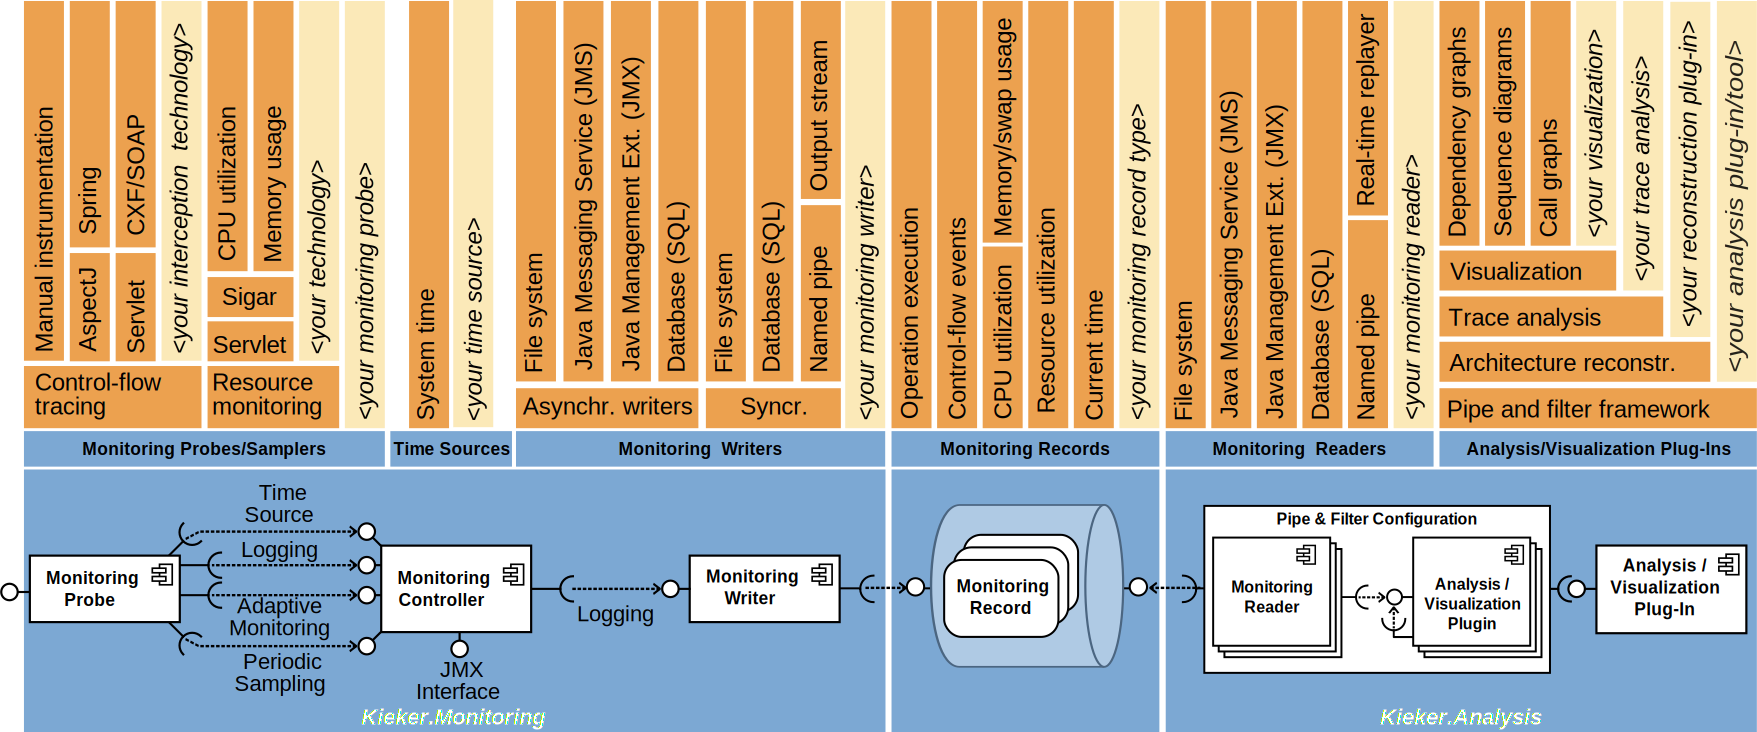
\includegraphics[width=\textwidth]{images/framework-figure}
\caption{Kieker framework components and extension points for custom components}
\label{fig:frameworkComponentsExtensionPoints}
\end{figure}

Figure~\ref{fig:frameworkComponentsExtensionPoints} depicts the possible %
extension points for custom components as well as the components which %
are already included in the \Kieker{} distribution and detailed below. %

\medskip

\begin{compactitem}
 \item \textbf{Monitoring writers and corresponding readers} for %
file systems and SQL databases, %
for in-memory record streams (named pipes), %
as well writers and readers employing Java Management %
Extensions (JMX)~\cite{JMX-Website} and %
Java Messaging Service~(JMS)~\cite{JMS-WebSite} technology. %
A special reader allows to replay existing persistent %
monitoring logs, for example to emulate incoming monitoring %
data---also in real-time.
 \item \textbf{Time sources} utilizing Java's \method{System.nanoTime()} (default) %
or \method{System.current\-TimeMillis()} methods.
 \item \textbf{Monitoring record types} allowing to store %
monitoring data about operation executions (including timing, control-flow, %
and session information), CPU and resource utilization, memory/swap usage, as well as %
a record type which can be used to store the current time.
\item \textbf{Monitoring probes}: A special feature of \Kieker{} is the ability to monitor (distributed) %
traces of method executions and corresponding timing information. %
For monitoring this data, Kieker includes monitoring probes employing %
AspectJ~\cite{AspectJ-WebSite}, %
Java~EE Servlet~\cite{JavaServletTechnology-WebSite}, %
Spring~\cite{Spring-WebSite}, and %
Apache~CXF~\cite{CXF-WebSite} technology. %
Additionally, Kieker includes probes for (periodic) system-level resource %
monitoring employing the Sigar library~\cite{HypericSigarWebsite}.
\item \textbf{Analysis/Visualization plugins} can be assembled to %
pipe-and-filter architectures based on input and output ports. The %
\KiekerTraceAnalysis{} tool 
% (Figure~\ref{fig:KiekerComponentDiagram}) %
% nie: Removed as this seems to be a wrong figure for this tool
is itself implemented based on a re-usable set of \KiekerAnalysisPart{} %
plugins allowing to reconstruct and visualize architectural models of the %
monitored systems, e.g., as dependency graphs, sequence diagrams, and call %
trees. %
\end{compactitem}



%%
% \pagebreak

\section{Licensing}

\Kieker{} is licensed under the Apache License, Version 2.0. You may obtain a copy of %
the license at \url{http://www.apache.org/licenses/LICENSE-2.0}.

The \Kieker{} source and binary release archives include a number of third-party %
libraries. %
% Appendix~\ref{appendix:libraries} lists these libraries along with information %
% on the licenses. 
The \dir{lib/} directory of the release archives contains a %
\file{.LICENSE} file for each third-party library, pointing to the respective license text.

\section{Citing Kieker}\label{sec:ch1:citingKieker}

When referencing Kieker resources in your publications, we would be happy if you %
respected the following guide lines:

\begin{itemize}
\item When referencing the Kieker project, please cite our %
ICPE~2012~\cite{KiekerICPE2012} paper and/or our 2009 technical report~\cite{vanHoornRohrHasselbringWallerEhlersFreyKieselhorst2009TRContinuousMonitoringOfSoftwareServicesDesignAndApplicationOfTheKiekerFramework}. %
Also, you might want to add a reference to our web site (\url{http://kieker-monitoring.net/}) %
like~\cite{KiekerWebSite}. 
\item When referencing this user guide, e.g., when reprinting contents, please %
use a citation like~\cite{KiekerUserGuideThis}.
\end{itemize}

\noindent At \url{http://kieker-monitoring.net/research/publications/} we provide %
entries for $\mathrm{B\scriptstyle IB}\!$\TeX{} and other bibliography %
systems.

\section{Kieker is Recommended by the SPEC Research Group}

In 2011, Kieker was reviewed and accepted for distribution as part of the SPEC Research %
Group's repository of peer-reviewed tools for quantitative system evaluation and analysis. %
See \url{http://research.spec.org/projects/tools.html} for details.

\section{Structure of this User Guide}

Based on a simple example, Chapter~\ref{chap:example} demonstrates %
how to manually instrument Java programs with \KiekerMonitoringPart{} %
in order to monitor timing information of method executions, and %
how to use \KiekerAnalysisPart{} to analyze the monitored data. %
Chapter~\ref{chap:componentsMonitoring} provides a more detailed %
description of \KiekerMonitoringPart{} and shows how to implement and %
use custom monitoring records, monitoring probes, and monitoring writers. %
A more detailed description of \KiekerAnalysisPart{} and how to implement and use %
custom monitoring readers, and analysis plugins follows in %
Chapter~\ref{chap:componentsAnalysis}. %
Chapter~\ref{chap:aspectJ} demonstrates how to use \KiekerTraceAnalysis{} %
for monitoring, analyzing, and visualizing trace information. %
Additional resources are included in the \hyperlink{hypertarget:appendix}{Appendix}, %
e.g., analyzing Java\,EE systems, using the JMS writers and readers, %
as well as monitoring system-level measures (CPU, memory, etc.) with %
Sigar. %

\vspace{1cm}

% Notify-tag because this could be interesting for the reader.
\NOTIFYBOX{The Java sources presented in this user guide, as well as pre-compiled binaries, %
are included in the %
\file{\exampleDir/} directory of the \Kieker{} distribution (see %
Section~\ref{sec:example:downloadInstall}). Also, the example directories can %
be imported as Eclipse projects.}


% \TODO{Point to Web site for additional examples, TR, \ldots}
